In  $\triangle LDO$
\begin{align}
\norm{\vec{O}-\vec{L}}+\norm{\vec{O}-\vec{D}}&=17.5> \norm{\vec{L}-\vec{D}}\\
\norm{\vec{O}-\vec{D}}+\norm{\vec{L}-\vec{D}}&=15>\norm{\vec{O}-\vec{L}}\\
\norm{\vec{O}-\vec{L}}+\norm{\vec{L}-\vec{D}}&=12.5>\norm{\vec{O}-\vec{D}}
\end{align}
and triangle inequality is satisfied.
%
Similarly, in $\triangle LDG$
\begin{align}
\norm{\vec{L}-\vec{D}} + \norm{\vec{G}-\vec{L}}&=11 > \norm{\vec{G}-\vec{D}}
\\
\norm{\vec{G}-\vec{L}} + \norm{\vec{G}-\vec{D}}&=12 > \norm{\vec{L}-\vec{D}}
\\
\norm{\vec{L}-\vec{D}} + \norm{\vec{G}-\vec{D}}&=11 > \norm{\vec{G}-\vec{L}}
\end{align}
and triangle inequality is satisfied.  
$\therefore$ the given sides form a quadrilateral which can be constructed by
using the approach in Problem \ref{const:tri_sss} to obtain the vertices of $\triangle LDO$ and 
$\triangle LDG$ as
\begin{align}
\vec{L}=\myvec{0\\0},\vec{D} = \myvec{5\\0}, \vec{O}=\myvec{-1.875\\7.26},\vec{G}=\myvec{2.5\\5.5}
\end{align}
and plotting the quadrilateral GOLD  in Fig. \ref{constr/34/fig:Quadrilateral GOLD}
%
\begin{figure}[!ht]
    \centering
    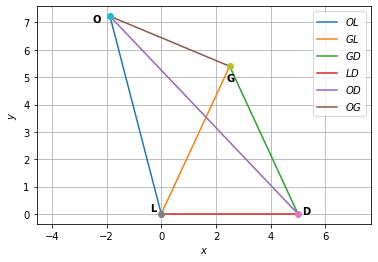
\includegraphics[width=\columnwidth]{solutions/34/GOLDfig.png}
    \caption{Quadrilateral GOLD}
    \label{constr/34/fig:Quadrilateral GOLD}
\end{figure}


